\documentclass{beamer}
\usepackage{tikz,amsmath,hyperref,graphicx,stackrel}
\usetikzlibrary{positioning,shadows,arrows,shapes,calc}
\newcommand{\argmax}{\operatornamewithlimits{argmax}}
\newcommand{\argmin}{\operatornamewithlimits{argmin}}
\mode<presentation>{\usetheme{Frankfurt}}
\AtBeginSection[]
{
  \begin{frame}<beamer>
    \frametitle{Outline}
    \tableofcontents[currentsection,currentsubsection]
  \end{frame}
}
\title{Lecture 10: Multivariate Gaussians}
\author{Mark Hasegawa-Johnson}
\date{ECE 417: Multimedia Signal Processing, Fall 2021}  
\begin{document}

% Title
\begin{frame}
  \maketitle
\end{frame}

% Title
\begin{frame}
  \tableofcontents
\end{frame}

%%%%%%%%%%%%%%%%%%%%%%%%%%%%%%%%%%%%%%%%%%%%
\section[Gaussians]{Gaussian Random Vectors}
\setcounter{subsection}{1}

\begin{frame}
  \frametitle{Gaussian (a.k.a. normal) pdf}
  \centerline{\includegraphics[height=2in]{exp/Normal_Distribution.png}}
  \begin{tiny}
    By InductiveLoad, public domain,
    \url{https://commons.wikimedia.org/wiki/File:Normal_Distribution_PDF.svg}
  \end{tiny}
\end{frame}

\begin{frame}
  \frametitle{Normal pdf}

  A Gaussian random variable, $X$, is one whose probability density
  function is given by
  \[
  f_X(x) = \frac{1}{\sqrt{2\pi\sigma^2}}e^{-\frac{1}{2}\frac{(x-\mu)^2}{\sigma^2}}
  \]
  where $\mu$ and $\sigma^2$ are the mean and variance,
  \[
  \mu=E\left[X\right],~~~
  \sigma^2 = E\left[(X-\mu)^2\right]
  \]
\end{frame}

\begin{frame}
  \frametitle{Standard normal}

  The cumulative distribution function (CDF) of a Gaussian RV is
  \[
  F_X(x)=P\left\{X\le x\right\}
  = \int_{-\infty}^x f_X(y)dy
  = \int_{-\infty}^{(x-\mu)/\sigma} f_Z(y)dy
  = \Phi\left(\frac{x-\mu}{\sigma}\right)
  \]
  where $Z=\frac{X-\mu}{\sigma}$ is called the standard normal random
  variable.  It  is a Gaussian with zero mean, and unit variance:
  \[
  f_Z(z) = \frac{1}{\sqrt{2\pi}}e^{-\frac{1}{2}z^2}
  \]
  We define $\Phi(z)$  to be the CDF of the standard normal RV:
  \[
  \Phi(z) =  \int_{-\infty}^{z} f_Z(y)dy
  \]
\end{frame}

\begin{frame}
  \frametitle{Multivariate normal pdf}
  \centerline{\includegraphics[height=2in]{exp/MultivariateNormal.png}}
  \begin{tiny}
    By Bscan, public domain,
    \url{https://commons.wikimedia.org/wiki/File:MultivariateNormal.png}
  \end{tiny}
\end{frame}

\begin{frame}
  \frametitle{Scalar Gaussian random variables}
  \[
  \mu=E[X],~~~\sigma^2=E[(X-\mu)^2]
  \]
  \centerline{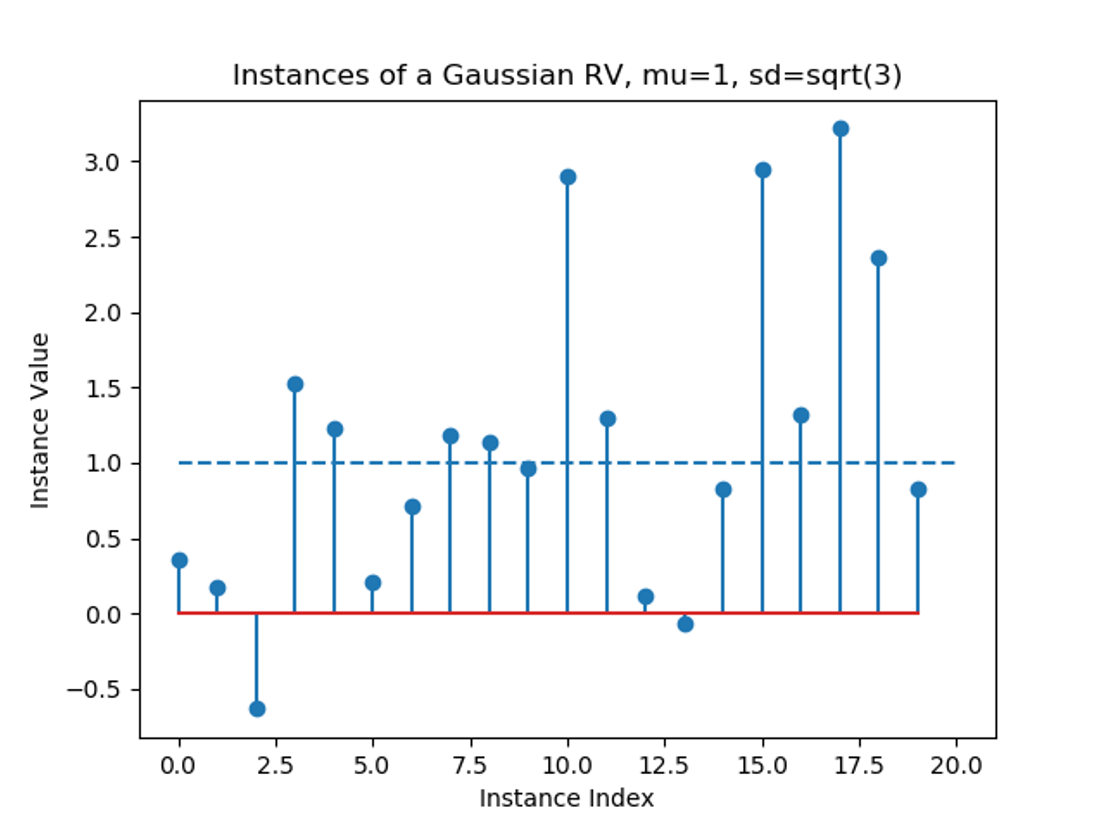
\includegraphics[height=3in]{gaussian_instances.png}}
\end{frame}

\begin{frame}
  \frametitle{Jointly Gaussian Random Variables}

  Two random variables, $X_1$ and $X_2$, are jointly Gaussian if
  \[
  f_{X_1,X_2}(x_1,x_2) = \frac{1}{2\pi|\Sigma|^{1/2}}
  e^{-\frac{1}{2}(\vec{x}-\vec\mu)^T\Sigma^{-1}(\vec{x}-\vec\mu)}
  \]
  where $\vec{X}$ is the random vector, $\vec\mu$ is its mean, and $\Sigma$ is its
  covariance matrix,
  \[
  \vec{X}=\left[\begin{array}{c}X_1\\X_2\end{array}\right],~~~
  \vec\mu=E\left[\vec{X}\right],~~~
  \Sigma = E\left[(\vec{X}-\vec\mu)^T(\vec{X}-\vec\mu)\right]
  \]
\end{frame}

\begin{frame}
  \begin{columns}
    \column{2.125in}
    \begin{block}{Gaussian random vector}
      \[
      \vec{x}=\left[\begin{array}{c}x_0\\\cdots\\x_{D-1}\end{array}\right]
      \]
      \[
      \vec\mu=E[\vec{x}]=\left[\begin{array}{c}\mu_0\\\cdots\\\mu_{D-1}\end{array}\right]
      \]
    \end{block}
    \column{2.125in}
    \begin{block}{Example: Instances of a Gaussian random vector}
      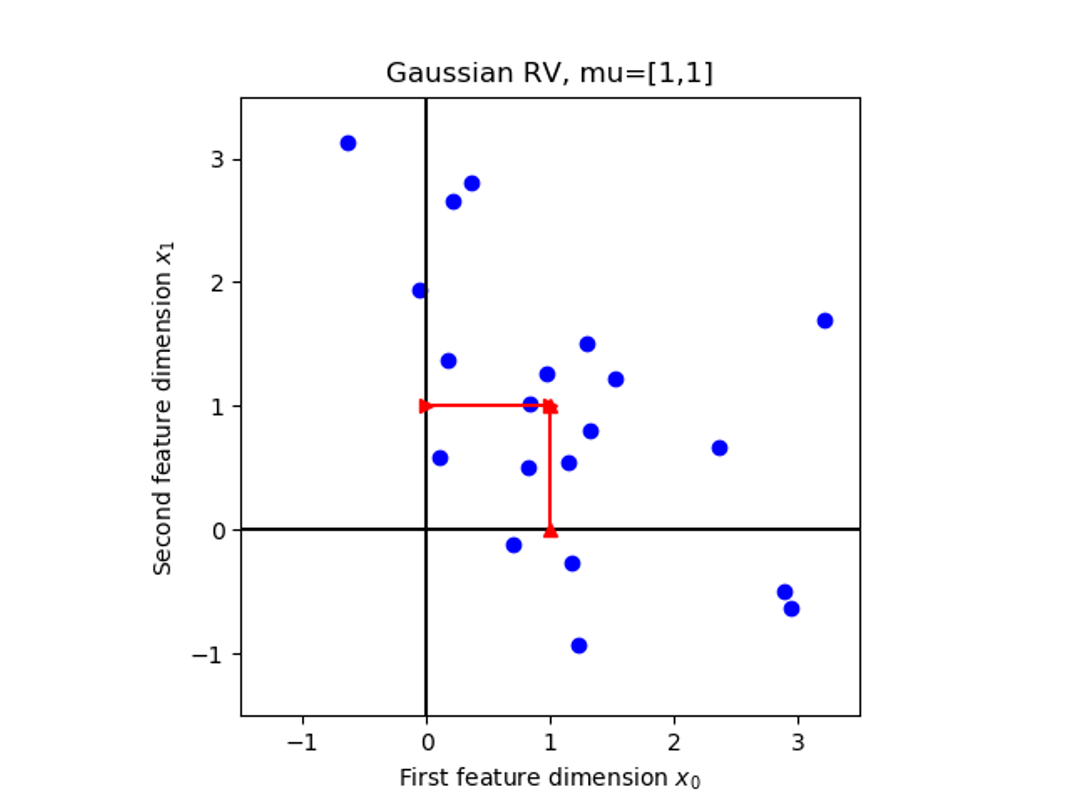
\includegraphics[width=2.1in]{gaussian_vectors.png}
    \end{block}
  \end{columns}
\end{frame}

\begin{frame}
  \frametitle{Covariance}
  The covariance matrix has four elements:
  \[
  \Sigma = \left[\begin{array}{cc}\sigma_1^2 & \rho_{12} \\\rho_{21} & \sigma_2^2\end{array}\right]
  \]
  $\sigma_1^2$ and $\sigma_2^2$ are the variances of $X_1$ and $X_2$, respectively.
  $\rho_{12}=\rho_{21}$ is the covariance of $X_1$ and $X_2$:
  \begin{align*}
    \mu_1 & = E[X_1]\\
    \sigma_1^2 &= E\left[(X_1-\mu_1)^2\right]\\
    \sigma_2^2 &= E\left[(X_2-\mu_2)^2\right]\\
    \rho_{12} &= E\left[(X_1-\mu_1)(X_2-\mu_2)\right]
  \end{align*}
\end{frame}

\begin{frame}
  \begin{columns}
    \column{2.25in}
    \begin{block}{Gaussian random vector}
      \[
      \Sigma= \left[\begin{array}{ccc}
          \sigma_0^2 & \rho_{01} & \ddots\\
          \rho_{10} & \ddots &  \rho_{D-2,D-1}\\
          \ddots & \rho_{D-1,D-2} &  \sigma_{D-1}^2\end{array}\right]
      \]
      where
      \[
      \rho_{ij}=E[(x_i-\mu_i)(x_j-\mu_j)]
      \]
      \[
      \sigma_{i}^2=E[(x_i-\mu_i)^2]
      \]
    \end{block}
    \column{2in}
    \begin{block}{Example: Instances of a Gaussian random vector}
      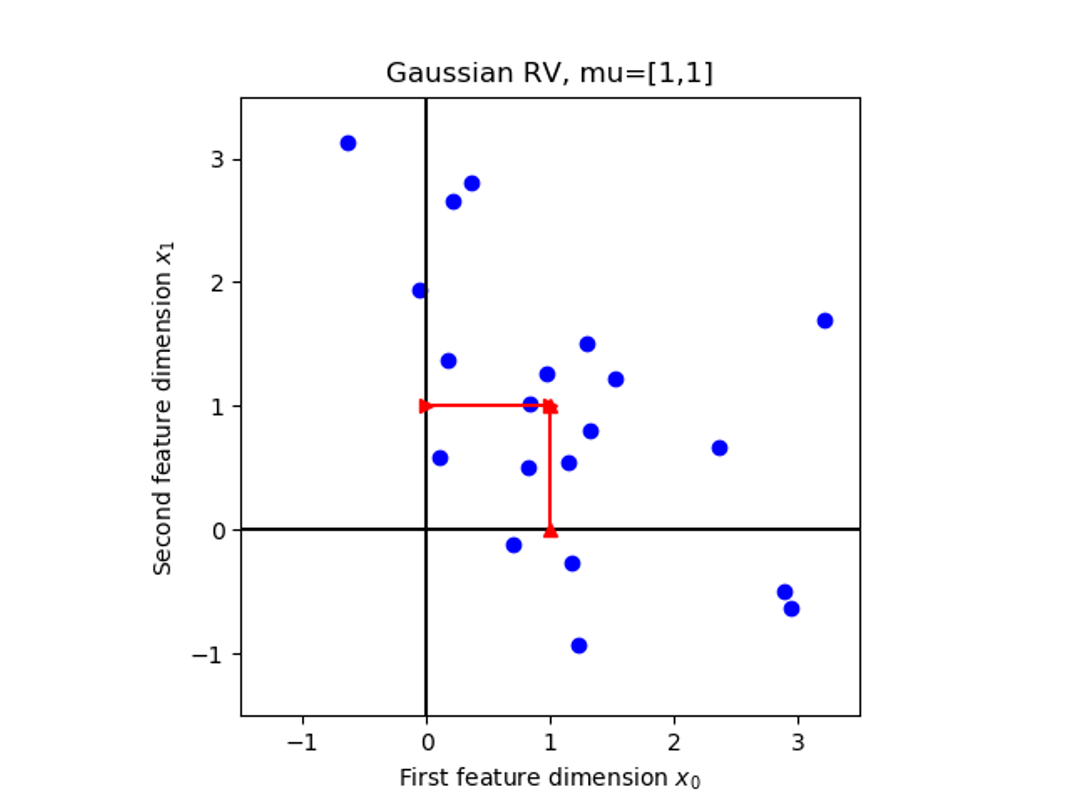
\includegraphics[width=1.9in]{gaussian_vectors.png}
    \end{block}
  \end{columns}
\end{frame}

\begin{frame}
  \frametitle{Jointly Gaussian Random Variables}
  \[
  f_{X_1,X_2}(x_1,x_2) = \frac{1}{2\pi|\Sigma|^{1/2}}
  e^{-\frac{1}{2}(\vec{x}-\vec\mu)^T\Sigma^{-1}(\vec{x}-\vec\mu)}
  \]
  The multivariate normal pdf contains the determinant and the inverse of $\Sigma$.
  For a two-dimensional vector $\vec{X}$, these are
  \begin{align*}
    \Sigma &= \left[\begin{array}{cc}\sigma_1^2 & \rho_{12} \\\rho_{21} & \sigma_2^2\end{array}\right]\\
    |\Sigma| &=\sigma_1^2\sigma_2^2 - \rho_{12}\rho_{21}\\
    \Sigma^{-1} &= \frac{1}{|\Sigma|}\left[\begin{array}{cc}
        \sigma_2^2 & -\rho_{12}\\-\rho_{21} & \sigma_1^2\end{array}\right]
  \end{align*}
\end{frame}  
  
\begin{frame}
  \frametitle{Gaussian: Uncorrelated $\Leftrightarrow$ Independent}

  Notice that if two Gaussian random variables are uncorrelated
  ($\rho_{12}=0$), then they are also independent:
  \begin{align*}
    f_{X_1,X_2}(x_1,x_2)
    &=\frac{1}{2\pi|\Sigma|^{1/2}}
    e^{-\frac{1}{2}
      \frac{\left[\begin{array}{c}x_1-\mu_1\\x_2-\mu_2\end{array}\right]^T
        \left[\begin{array}{cc}\sigma_2^2&0\\0&\sigma_1^2\end{array}\right]
        \left[\begin{array}{c}x_1-\mu_1\\x_2-\mu_2\end{array}\right]}
      {\sigma_1^2\sigma_2^2}}\\
    &=\frac{1}{2\pi\sigma_1\sigma_2}
    e^{-\frac{1}{2}\left(\frac{(x_1-\mu_1)^2}{\sigma_1^2}+\frac{(x_2-\mu_2)^2}{\sigma_2^2}\right)}\\
    &=\left(\frac{1}{\sqrt{2\pi\sigma_1^2}}e^{-\frac{1}{2}\left(\frac{x_1-\mu_2}{\sigma_1}\right)^2}\right)
    \left(\frac{1}{\sqrt{2\pi\sigma_2^2}}e^{-\frac{1}{2}\left(\frac{x_2-\mu_2}{\sigma_2}\right)^2}\right)
    \\
    &=f_{X_1}(x_1)f_{X_2}(x_2)
  \end{align*}
\end{frame}  

\begin{frame}
  \begin{columns}
    \column{2.25in}
    \begin{block}{Sample Mean, Sample Covariance}
      In the real world, we don't know $\vec\mu$ and $\Sigma$!
      If we have $M$  instances $\vec{x}_m$  of the Gaussian,
      we can estimate
      \[
      \vec\mu=\frac{1}{M}\sum_{m=0}^{M-1}\vec{x}_m
      \]
      \[
      \Sigma=\frac{1}{M-1}\sum_{m=0}^{M-1}(\vec{x}_m-\vec\mu)(\vec{x}_m-\vec\mu)^T
      \]
      Sample mean and sample covariance are not the same as real mean
      and real covariance, but we'll use the same letters ($\vec\mu$
      and $\Sigma$) unless the problem requires us to distinguish.
    \end{block}
    \column{2in}
    \begin{block}{Examples of $\vec{x}_m-\vec\mu$}
      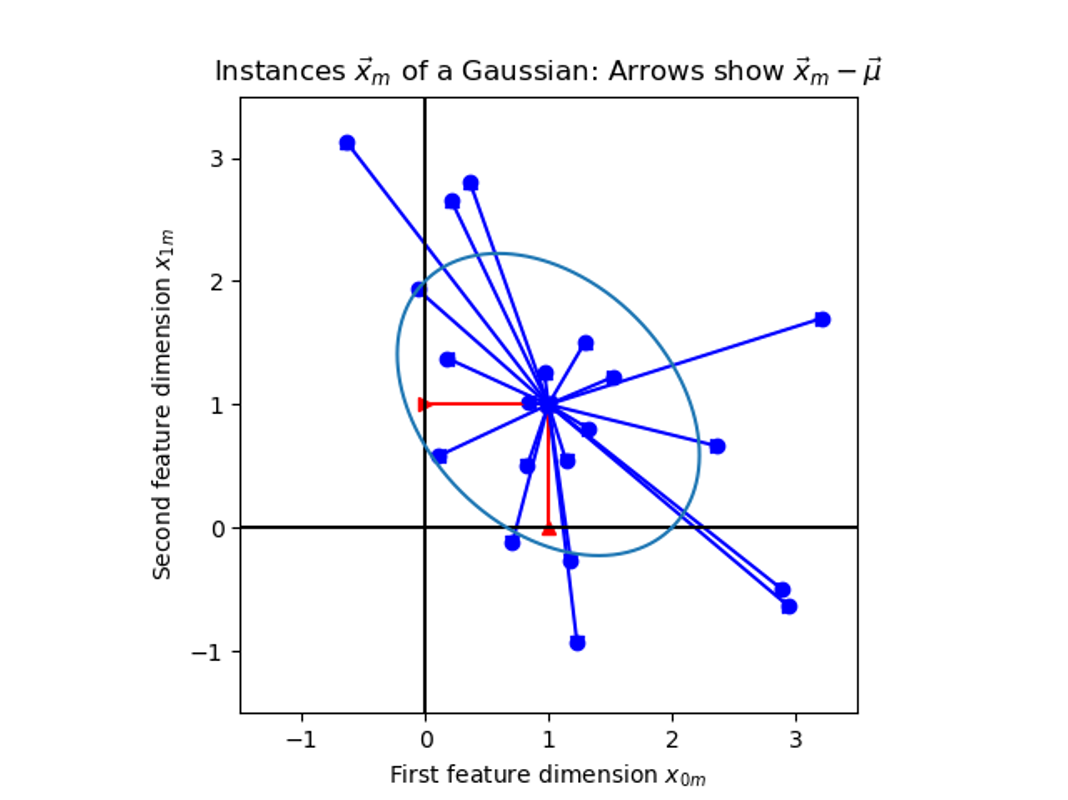
\includegraphics[width=1.9in]{gaussian_subtraction.png}
    \end{block}
  \end{columns}
\end{frame}

%%%%%%%%%%%%%%%%%%%%%%%%%%%%%%%%%%%%%%%%%%%%
\section[PCA]{Principal Components}
\setcounter{subsection}{1}

\begin{frame}
  \begin{columns}
    \column{2.25in}
    \begin{block}{Sample covariance}
      \begin{align*}
        \Sigma&=\frac{1}{M-1}\sum_{m=0}^{M-1}(\vec{x}_m-\vec\mu)(\vec{x}_m-\vec\mu)^T\\
        &=\frac{1}{M-1}X^TX
      \end{align*}
      \ldots where $X$ is the centered data matrix,
      \[
      X=\left[\begin{array}{c}
          (\vec{x}_0-\vec\mu)^T\\\vdots\\(\vec{x}_{M-1}-\vec\mu)^T\end{array}\right]
      \]
    \end{block}
    \column{2.125in}
    \begin{block}{Examples of $\vec{x}_m-\vec\mu$}
      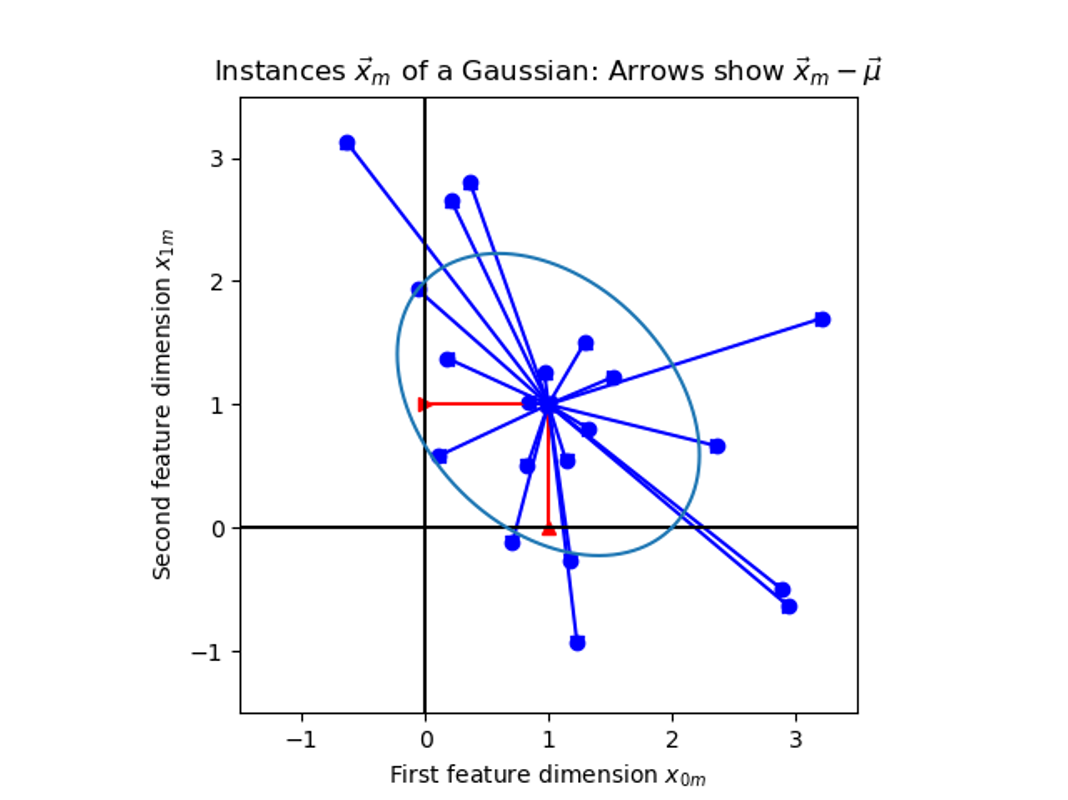
\includegraphics[width=2.1in]{gaussian_subtraction.png}
    \end{block}
  \end{columns}
\end{frame}

\begin{frame}
  \begin{columns}
    \column{1.75in}
    \begin{block}{Centered data matrix}
      \[
      X=\left[\begin{array}{c}
          (\vec{x}_0-\vec\mu)^T\\\vdots\\(\vec{x}_{M-1}-\vec\mu)^T\end{array}\right]
      \]
    \end{block}
    \column{2.625in}
    \begin{block}{Examples of $\vec{x}_m-\vec\mu$}
      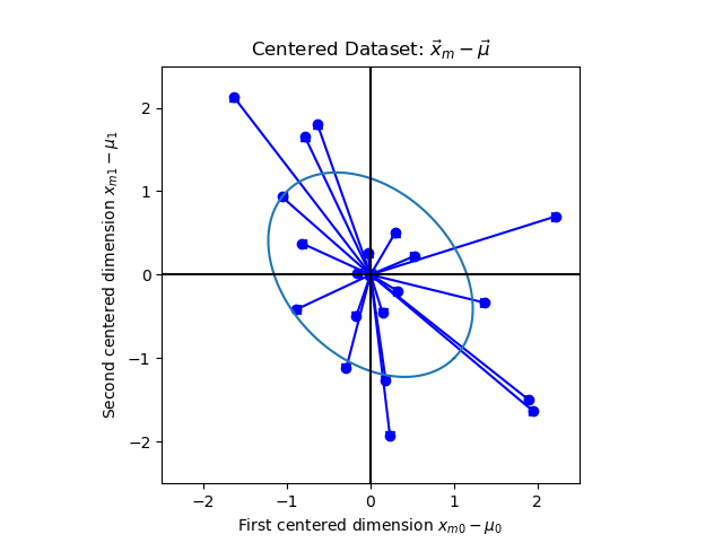
\includegraphics[width=2.5in]{centered_data.png}
    \end{block}
  \end{columns}
\end{frame}

\begin{frame}
  \begin{columns}
    \column{1.75in}
    \begin{block}{Principal component axes}
      $X^TX$ is symmetric!  Therefore,
      \[
      X^TX=V\Lambda V^T
      \]
      $V=[\vec{v}_0,\ldots,\vec{v}_{D-1}]$, the eigenvectors
      of $X^TX$, are called the principal component axes,
      or principal component directions.
    \end{block}
    \column{2.625in}
    \begin{block}{Principal component axes}
      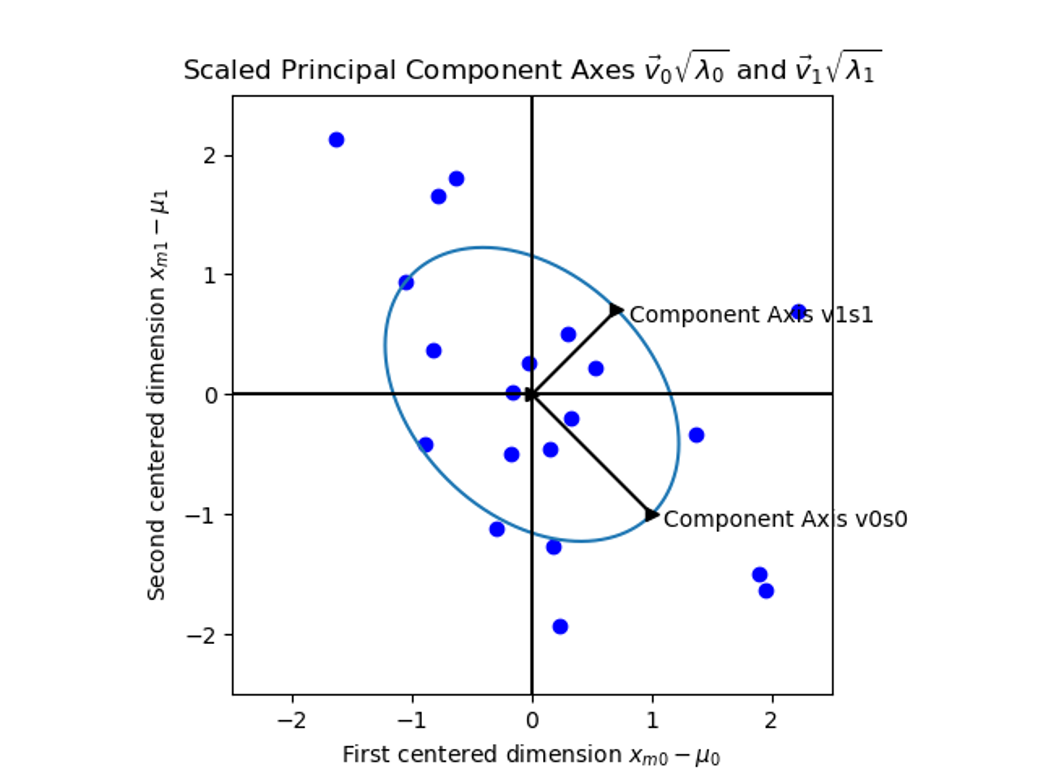
\includegraphics[width=2.5in]{principal_component_axes.png}
    \end{block}
  \end{columns}
\end{frame}

\begin{frame}
  \frametitle{Principal components}
  Remember that the eigenvectors of a matrix diagonalize it.
  So if $V$ are the eigenvectors of $X^TX$, then
  \[
  V^TX^TXV=\Lambda
  \]
  Let's write $Y=XV$, and $Y^T=V^TX^T$.  In other words,
  \[
  \vec{y}_m=V^T(\vec{x}_m-\vec\mu)
  \]
  $\vec{y}_m=[y_{m0},\ldots,y_{m,D-1}]^T$ is the vector of
  principal components of $\vec{x}_m$.  Expanding the formula
  $Y^TY=\Lambda$, we discover that PCA orthogonalizes the dataset:
  \[
  \sum_{m=0}^{M-1}y_{im}y_{jm}=\begin{cases}
  \lambda_i & i=j\\0&i\ne j
  \end{cases}
  \]
\end{frame}

\begin{frame}
  \frametitle{Principal components}
  \[
  \vec{y}_m=V^T(\vec{x}_m-\vec\mu)
  \]
  \centerline{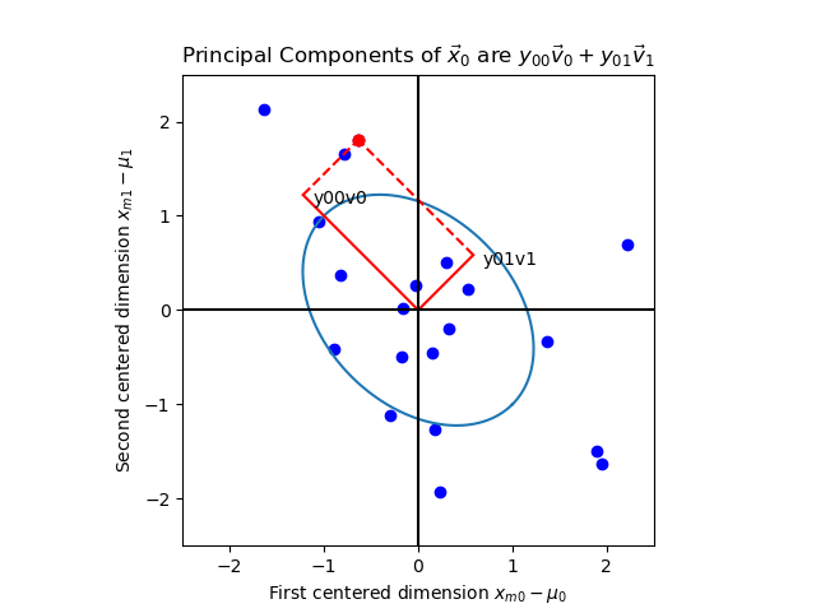
\includegraphics[height=3in]{principal_components.png}}
\end{frame}

\begin{frame}
  \frametitle{Principal components with larger eigenvalues have more energy}
  \centerline{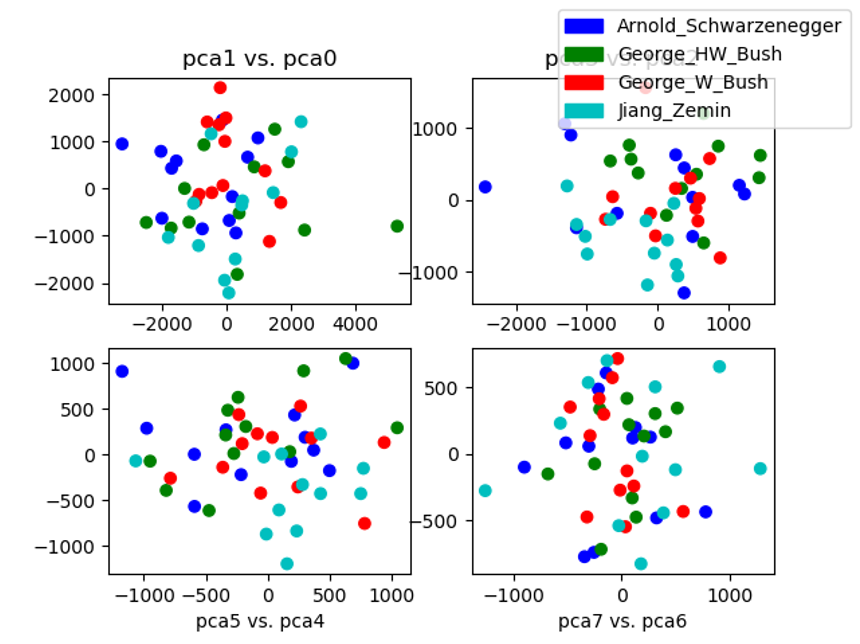
\includegraphics[height=3in]{pca_samples.png}}
\end{frame}

\begin{frame}
  \frametitle{Eigenvalue=Energy of the Principal Component}
  The total dataset energy is
  \[
  \sum_{m=0}^{M-1}y_{mi}^2=\lambda_i
  \]
  But remember that $V^TV=I$.  Therefore, the total dataset energy
  is the same, whether you calculate it in the original image
  domain, or in the PCA domain:
  \[
  \sum_{m=0}^{M-1}\sum_{d=0}^{D-1}(x_{md}-\mu_d)^2
  =\sum_{m=0}^{M-1}\sum_{i=0}^{D-1}y_{mi}^2=\sum_{i=0}^{D-1}\lambda_i
  \]
\end{frame}

\begin{frame}
  \frametitle{Energy  spectrum=Fraction of energy explained}
  The ``energy spectrum'' is energy as a function of
  basis vector index.  There are a few ways we could define it,
  but one useful definition is:
  \begin{align*}
    E[k] &=\frac{\sum_{m=0}^{M-1}\sum_{i=0}^{k-1}y_{mi}^2}
    {\sum_{m=0}^{M-1}\sum_{i=0}^{D-1}y_{mi}^2}\\
    &=\frac{\sum_{i=0}^{k-1}\lambda_i}{\sum_{i=0}^{D-1}\lambda_i}
  \end{align*}
\end{frame}

\begin{frame}
  \frametitle{Energy  spectrum=Fraction of energy explained}
  \centerline{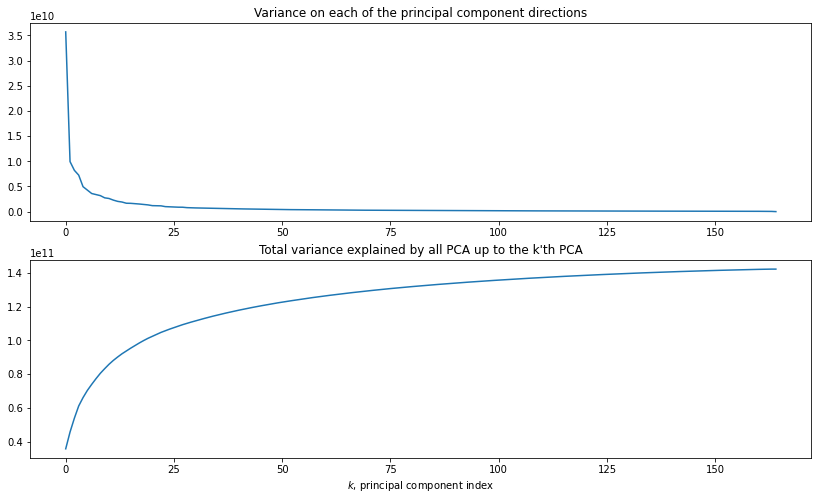
\includegraphics[height=3in]{energy_spectrum.png}}
\end{frame}


%%%%%%%%%%%%%%%%%%%%%%%%%%%%%%%%%%%%%%%%%%%%
\section[SVD]{Singular Value Decomposition}
\setcounter{subsection}{1}

\begin{frame}
  \begin{columns}
    \column{2.125in}
    \begin{block}{Gram matrix}
      \begin{itemize}
      \item $X^TX$ is usually called the sum-of-squares matrix.
        $\frac{1}{M-1}X^TX$ is the sample covariance.
      \item $G=XX^T$ is called the gram matrix.
        Its $(i,j)^{\textrm{th}}$ element is the dot product between
        the $i^{\textrm{th}}$ and $j^{\textrm{th}}$ data samples:
        \[
        g_{ij}=(\vec{x}_i-\vec\mu)^T(\vec{x}_j-\vec\mu)
        \]
      \end{itemize}
    \end{block}
    \column{2.125in}
    \begin{block}{Gram matrix $g_{01}=(\vec{x}_0-\vec\mu)^T(\vec{x}_1-\vec\mu)$}
      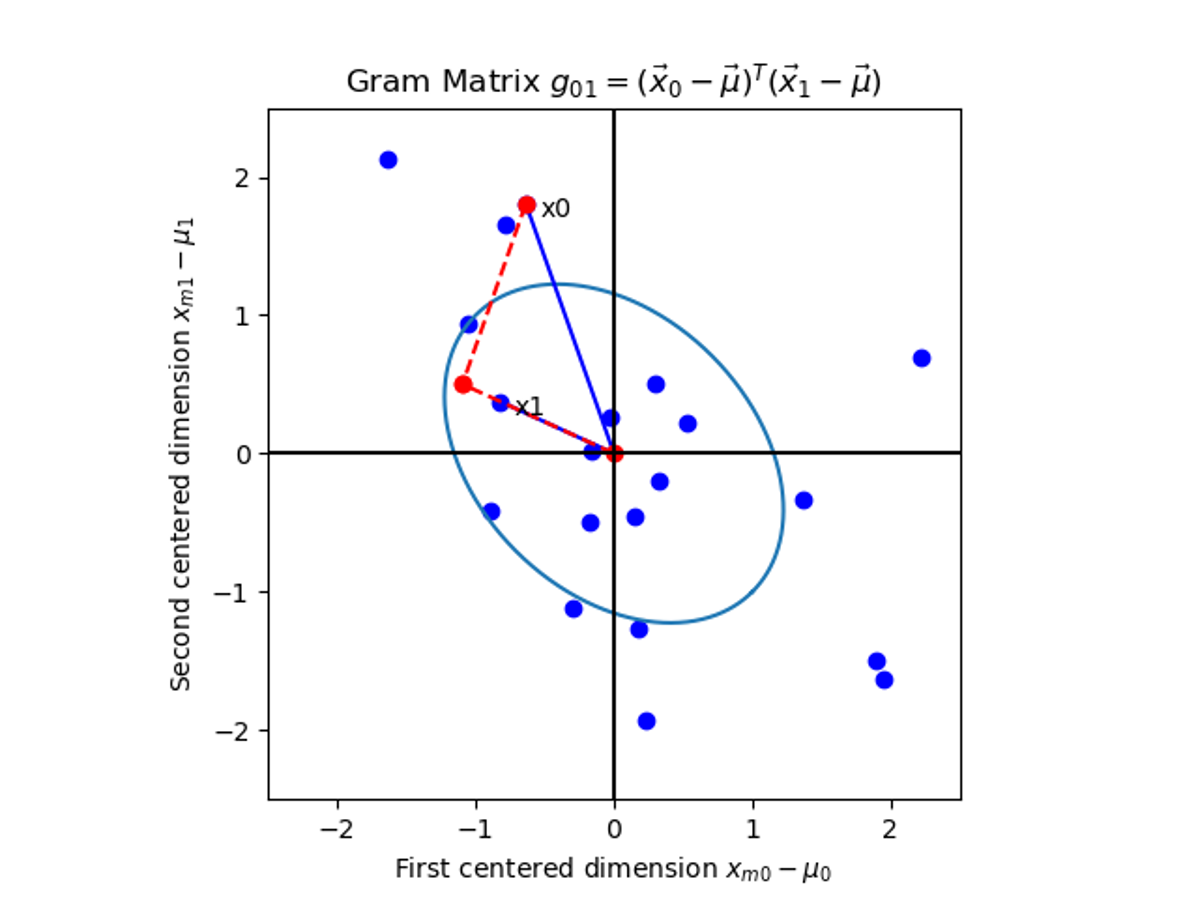
\includegraphics[width=2.1in]{gram_matrix.png}
    \end{block}
  \end{columns}
\end{frame}

\begin{frame}
  \begin{columns}
    \column{2.125in}
    \begin{block}{Eigenvectors of the Gram matrix}
      $XX^T$ is also symmetric!  So it has orthonormal eigenvectors:
      \[
      XX^T=U\Lambda U^T
      \]
      \[
      UU^T=U^TU=I
      \]
      $X^TX$ and $XX^T$ have the same eigenvalues ($\Lambda$),
      but different eigenvectors ($V$ vs. $U$).
    \end{block}
    \column{2.125in}
    \begin{block}{Gram matrix $g_{01}=(\vec{x}_0-\vec\mu)^T(\vec{x}_1-\vec\mu)$}
      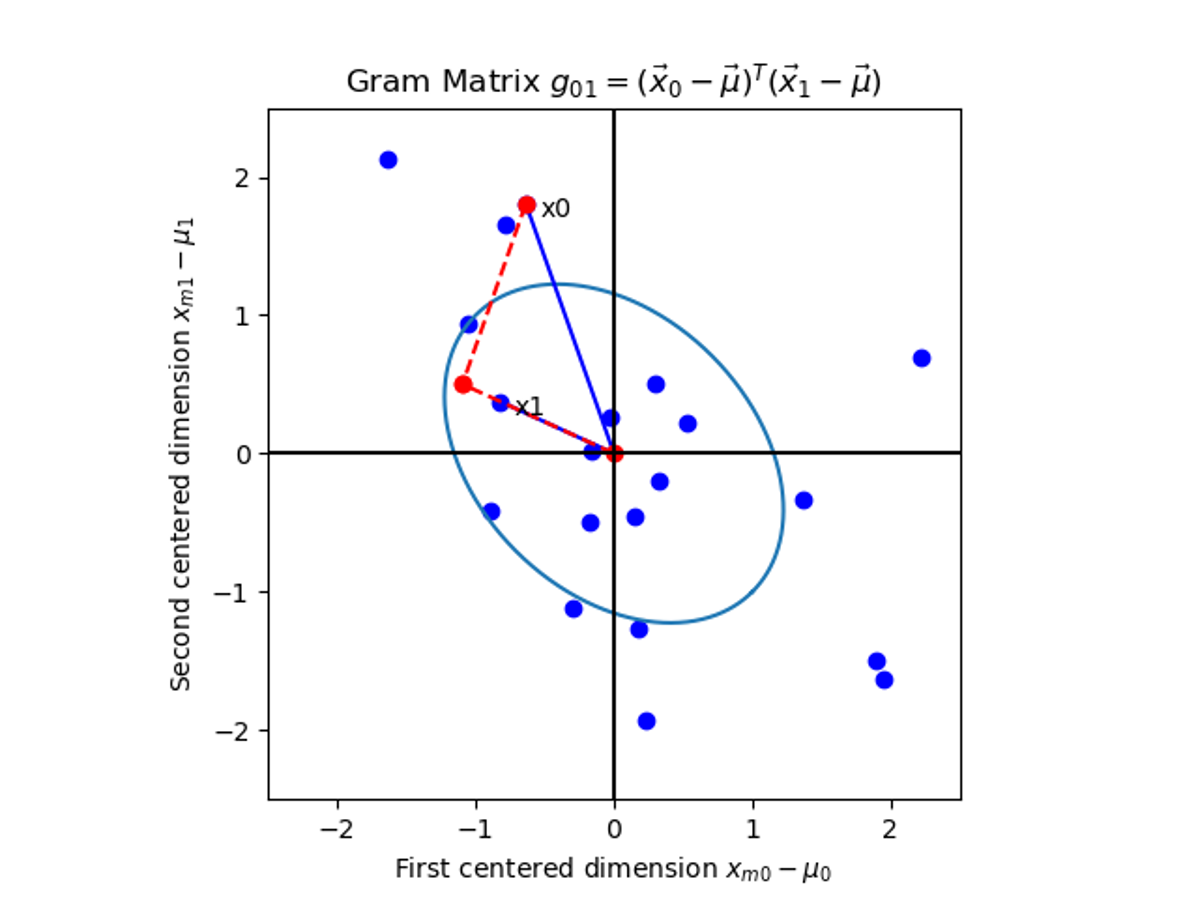
\includegraphics[width=2.1in]{gram_matrix.png}
    \end{block}
  \end{columns}
\end{frame}

\begin{frame}
  \frametitle{Why the Gram matrix is useful:}

  Suppose (as in MP1) that $D\sim 240000$ pixels per image, but $M\sim
  240$ different images.  Then, in order to perform this eigenvalue
  analysis:
  \[
  X^TX = V\Lambda V^T
  \]
  \ldots requires factoring a $240000^{\textrm{th}}$-order polynomial
  ($|X^TX-\lambda I|=0$), then solving 240000 simultaneous linear
  equations in 240000 unknowns to find each eigenvector
  ($X^TX\vec{v}_d=\lambda_d\vec{v}_d$).  If you try doing that using
  {\tt np.linalg.eig}, your PC will be running all day.  On the other
  hand,
  \[
  XX^T=U\Lambda U^T
  \]
  requires only 240 equations in 240 unknowns.  Educated experts
  agree: $240^2 \ll 240000^2$.
\end{frame}
  
\begin{frame}
  \frametitle{Singular Values}
  \begin{itemize}
  \item Both $X^TX$ and $XX^T$ are positive semi-definite, meaning
    that their eigenvalues are non-negative, $\lambda_d\ge 0$.
  \item The {\bf singular values} of $X$ are defined to be the
    square roots of the eigenvalues of $X^TX$ and $XX^T$:
    \[
    S=\left[\begin{array}{ccc}s_0&0&0\\0&\ldots&0\\0&0&s_{D-1}\end{array}\right],~~~
    \Lambda=S^2=\left[\begin{array}{ccc}s_0^2&0&0\\0&\ldots&0\\0&0&s_{D-1}^2\end{array}\right]
    \]
  \end{itemize}
\end{frame}

\begin{frame}
  \frametitle{Singular Value Decomposition}
  \[
  X^TX=V\Lambda V^T = VSSV^T
  \]
  \[
  XX^T=U\Lambda U^T = USSU^T
  \]
\end{frame}

\begin{frame}
  \frametitle{Singular Value Decomposition}
  \[
  X^TX= VSSV^T= VSISV^T= VSU^TUSV^T = (USV^T)^T(USV^T)
  \]
  \[
  XX^T= USSU^T= USISU^T= USV^TVSU^T = (USV^T)(USV^T)^T
  \]
\end{frame}

\begin{frame}
  \frametitle{Singular Value Decomposition}
  Any matrix, $X$, can be written as $X=USV^T$.
  \begin{itemize}
  \item $U=[\vec{u}_0,\ldots,\vec{u}_{M-1}]$ are the eigenvectors of $XX^T$.
  \item $V=[\vec{v}_0,\ldots,\vec{v}_{D-1}]$ are the eigenvectors of $X^TX$.
  \item $S=\left[\begin{array}{ccccc}s_0&0&0&0&0\\0&\ldots&0&0&0\\0&0&s_{\min(D,M)-1}&0&0\end{array}\right]$ are the singular values.
  \end{itemize}
  $S$ has some all-zero columns if $M>D$, or all-zero rows if $M<D$.
\end{frame}

\begin{frame}
  \frametitle{What np.linalg.svd does}
  First, {\tt np.linalg.svd} decides whether it wants to find the eigenvectors of
  $X^TX$ or $XX^T$: it just checks to see whether $M>D$ or vice versa.
  If it discovers that $M<D$, then:
  \begin{enumerate}
  \item Compute  $XX^T=U\Lambda U^T$, and $S=\sqrt{\Lambda}$.
    Now we have $U$ and $S$, we just need to  find $V$.
  \item Since $X^T=VSU^T$, we can get $V$ by just multiplying:
    \[
    \tilde{V} = X^TU
    \]
    \ldots where $\tilde{V}=VS$ is exactly equal to $V$, but with each column
    scaled by a different singular value.  So we just need to normalize:
    \[
    \Vert\vec{v}_i\Vert=1,~~~v_{i0}>0
    \]
  \end{enumerate}
\end{frame}

\begin{frame}
  \frametitle{Methods that solve MP1}
  \begin{itemize}
  \item Direct eigenvector analysis of $X^TX$ gives the right answer, but
    takes a very long time. When I tried this, it timed out the autograder.
  \item Applying {\tt np.linalg.svd} to $X$ should give the right answer, very fast.
    I haven't tried it this year, but it worked on last year's dataset.
  \item What I tried, this year, is the gram matrix method: Apply {\tt
    np.linalg.eig} to get $U$ from $XX^T$. Multiply $\tilde{V}=X^TU$,
    then normalize the columns to get $V$.
  \end{itemize}
\end{frame}

%%%%%%%%%%%%%%%%%%%%%%%%%%%%%%%%%%%%%%%%%%%%%%%%%%%%%%%%%%%%%%%%%%%%%%%%%%%%%%%%%%%%%
\section{Summary}
\setcounter{subsection}{1}

\begin{frame}
  \frametitle{Summary}
\end{frame}

\end{document}

